\documentclass[aspectratio=169]{beamer}

\usetheme{Boadilla}
\usefonttheme{professionalfonts}
\setbeamertemplate{navigation symbols}{}
\setbeamertemplate{itemize items}[circle]
\setbeamertemplate{enumerate items}[default]
\setbeamertemplate{headline}{}

\usepackage[utf8]{inputenc}
\usepackage[T1]{fontenc}
\usepackage{lmodern}
\usepackage{amsmath}
\usepackage{booktabs}
\usepackage{tabularx}
\usepackage{array}
\usepackage{hyperref}
\usepackage[strings]{underscore}
\usepackage{listings}
\usepackage{tikz}
\usetikzlibrary{arrows.meta,positioning,fit,calc,shapes.geometric}
\usepackage{xcolor}

\definecolor{courseblue}{HTML}{12355B}
\definecolor{coursegold}{HTML}{C98A2E}
\definecolor{courseice}{HTML}{EEF3F8}
\definecolor{coursegreen}{HTML}{2F6B4F}
\definecolor{coursegray}{HTML}{4B5563}
\definecolor{codebg}{HTML}{F7F9FC}
\definecolor{codecomment}{HTML}{5E6C84}
\definecolor{codestring}{HTML}{0B6E4F}

\setbeamercolor{palette primary}{bg=courseblue,fg=white}
\setbeamercolor{palette secondary}{bg=coursegold,fg=white}
\setbeamercolor{palette tertiary}{bg=courseblue,fg=white}
\setbeamercolor{palette quaternary}{bg=coursegold,fg=white}
\setbeamercolor{structure}{fg=courseblue}
\setbeamercolor{frametitle}{bg=courseice,fg=courseblue}
\setbeamercolor{title}{fg=courseblue}
\setbeamercolor{block title}{bg=courseblue,fg=white}
\setbeamercolor{block body}{bg=courseice,fg=black}
\setbeamercolor{normal text}{fg=black,bg=white}
\setbeamercolor{alerted text}{fg=coursegold}

\setbeamerfont{footline}{size=\scriptsize}

\setbeamertemplate{footline}{
  \leavevmode
  \hbox{
    \begin{beamercolorbox}[wd=.33\paperwidth,ht=2.8ex,dp=1.2ex,leftskip=0.8em]{palette primary}%
      University of Trieste
    \end{beamercolorbox}%
    \begin{beamercolorbox}[wd=.49\paperwidth,ht=2.8ex,dp=1.2ex,center]{palette tertiary}%
      \coursename{} \textbar{} \coursecode
    \end{beamercolorbox}%
    \begin{beamercolorbox}[wd=.18\paperwidth,ht=2.8ex,dp=1.2ex,rightskip=0.8em plus1fil]{palette secondary}%
      \insertframenumber{} / \inserttotalframenumber
    \end{beamercolorbox}%
  }
}

\hypersetup{
  colorlinks=true,
  linkcolor=courseblue,
  urlcolor=coursegreen
}

\lstdefinestyle{coursepython}{
  language=Python,
  basicstyle=\ttfamily\footnotesize,
  keywordstyle=\color{courseblue}\bfseries,
  commentstyle=\color{codecomment}\itshape,
  stringstyle=\color{codestring},
  showstringspaces=false,
  columns=fullflexible,
  keepspaces=true,
  frame=single,
  framerule=0.6pt,
  rulecolor=\color{courseblue},
  backgroundcolor=\color{codebg},
  xleftmargin=0.4em,
  xrightmargin=0.4em,
  aboveskip=0.4em,
  belowskip=0.2em
}

\newcommand{\coursename}{Data-driven Systems Engineering}
\newcommand{\coursecode}{440MI / 305SM}
\newcommand{\coursefooter}{}

\newcommand{\learninggoals}[1]{
  \begin{block}{Learning goals}
  #1
  \end{block}
}

\newcommand{\repoactivity}[1]{
  \begin{block}{Repo activity}
  #1
  \end{block}
}

\newcommand{\readinglist}[1]{
  \begin{block}{Papers and materials}
  {\footnotesize #1}
  \end{block}
}

\newcommand{\coursecontextframe}[5]{
  \begin{frame}{Course Map and Running Cases}
  \centering
  \begin{tikzpicture}[node distance=0.28cm]
  \node[flowbox, minimum width=1.45cm, minimum height=0.8cm] (problem) {\scriptsize Problem};
  \node[flowbox, minimum width=1.45cm, minimum height=0.8cm, right=of problem] (data) {\scriptsize Data};
  \node[flowbox, minimum width=1.45cm, minimum height=0.8cm, right=of data] (features) {\scriptsize Features};
  \node[flowbox, minimum width=1.45cm, minimum height=0.8cm, right=of features] (model) {\scriptsize Model};
  \node[flowbox, minimum width=1.45cm, minimum height=0.8cm, right=of model] (interface) {\scriptsize Interface};
  \node[flowbox, minimum width=1.45cm, minimum height=0.8cm, right=of interface] (delivery) {\scriptsize Delivery};
  \node[flowbox, minimum width=1.45cm, minimum height=0.8cm, right=of delivery] (monitor) {\scriptsize Monitor};
  \node[accentbox, minimum width=1.6cm, minimum height=0.8cm, right=of monitor] (evolution) {\scriptsize Evolution};
  \foreach \a/\b in {problem/data,data/features,features/model,model/interface,interface/delivery,delivery/monitor,monitor/evolution} {
    \draw[arrow] (\a) -- (\b);
  }
  \end{tikzpicture}

  \vspace{0.5em}
  \begin{block}{Today in the course}
  \textbf{Focus:} #1

  \textbf{Bridge:} #2
  \end{block}

  \begin{columns}[T]
  \column{0.48\textwidth}
  \begin{block}{Fraud case}
  {\footnotesize #3}
  \end{block}
  \column{0.48\textwidth}
  \begin{block}{Pasteurization case}
  {\footnotesize #4}
  \end{block}
  \end{columns}

  \vspace{0.3em}
  {\footnotesize \textbf{Course thread:} #5}
  \coursefooter
  \end{frame}
}

\newcommand{\classclosingframe}[4]{
  \begin{frame}{From This Class to the Next}
  \begin{block}{What stays with us}
  #1
  \end{block}

  \begin{columns}[T]
  \column{0.48\textwidth}
  \begin{block}{Project use}
  {\footnotesize #2}
  \end{block}
  \column{0.48\textwidth}
  \begin{block}{Next connection}
  {\footnotesize #3}
  \end{block}
  \end{columns}

  \vspace{0.3em}
  {\footnotesize \textbf{Course thread:} #4}
  \coursefooter
  \end{frame}
}

\tikzset{
  flowbox/.style={
    rounded corners=3pt,
    draw=courseblue,
    fill=courseice,
    very thick,
    minimum width=2.2cm,
    minimum height=0.9cm,
    align=center,
    font=\small
  },
  accentbox/.style={
    rounded corners=3pt,
    draw=coursegold,
    fill=coursegold!15,
    very thick,
    minimum width=2.2cm,
    minimum height=0.9cm,
    align=center,
    font=\small
  },
  arrow/.style={
    -{Latex[length=2.5mm,width=2mm]},
    thick,
    draw=courseblue
  }
}

% Visual layer on top of common.tex: tiles, icons, a progress-strip section divider, and a footer
% strip that defines the concepts appearing for the first time on each slide.
% Same look as the Class 20 deck. Load with:  \documentclass[aspectratio=169]{beamer}

\usetheme{Boadilla}
\usefonttheme{professionalfonts}
\setbeamertemplate{navigation symbols}{}
\setbeamertemplate{itemize items}[circle]
\setbeamertemplate{enumerate items}[default]
\setbeamertemplate{headline}{}

\usepackage[utf8]{inputenc}
\usepackage[T1]{fontenc}
\usepackage{lmodern}
\usepackage{amsmath}
\usepackage{booktabs}
\usepackage{tabularx}
\usepackage{array}
\usepackage{hyperref}
\usepackage[strings]{underscore}
\usepackage{listings}
\usepackage{tikz}
\usetikzlibrary{arrows.meta,positioning,fit,calc,shapes.geometric}
\usepackage{xcolor}

\definecolor{courseblue}{HTML}{12355B}
\definecolor{coursegold}{HTML}{C98A2E}
\definecolor{courseice}{HTML}{EEF3F8}
\definecolor{coursegreen}{HTML}{2F6B4F}
\definecolor{coursegray}{HTML}{4B5563}
\definecolor{codebg}{HTML}{F7F9FC}
\definecolor{codecomment}{HTML}{5E6C84}
\definecolor{codestring}{HTML}{0B6E4F}

\setbeamercolor{palette primary}{bg=courseblue,fg=white}
\setbeamercolor{palette secondary}{bg=coursegold,fg=white}
\setbeamercolor{palette tertiary}{bg=courseblue,fg=white}
\setbeamercolor{palette quaternary}{bg=coursegold,fg=white}
\setbeamercolor{structure}{fg=courseblue}
\setbeamercolor{frametitle}{bg=courseice,fg=courseblue}
\setbeamercolor{title}{fg=courseblue}
\setbeamercolor{block title}{bg=courseblue,fg=white}
\setbeamercolor{block body}{bg=courseice,fg=black}
\setbeamercolor{normal text}{fg=black,bg=white}
\setbeamercolor{alerted text}{fg=coursegold}

\setbeamerfont{footline}{size=\scriptsize}

\setbeamertemplate{footline}{
  \leavevmode
  \hbox{
    \begin{beamercolorbox}[wd=.33\paperwidth,ht=2.8ex,dp=1.2ex,leftskip=0.8em]{palette primary}%
      University of Trieste
    \end{beamercolorbox}%
    \begin{beamercolorbox}[wd=.49\paperwidth,ht=2.8ex,dp=1.2ex,center]{palette tertiary}%
      \coursename{} \textbar{} \coursecode
    \end{beamercolorbox}%
    \begin{beamercolorbox}[wd=.18\paperwidth,ht=2.8ex,dp=1.2ex,rightskip=0.8em plus1fil]{palette secondary}%
      \insertframenumber{} / \inserttotalframenumber
    \end{beamercolorbox}%
  }
}

\hypersetup{
  colorlinks=true,
  linkcolor=courseblue,
  urlcolor=coursegreen
}

\lstdefinestyle{coursepython}{
  language=Python,
  basicstyle=\ttfamily\footnotesize,
  keywordstyle=\color{courseblue}\bfseries,
  commentstyle=\color{codecomment}\itshape,
  stringstyle=\color{codestring},
  showstringspaces=false,
  columns=fullflexible,
  keepspaces=true,
  frame=single,
  framerule=0.6pt,
  rulecolor=\color{courseblue},
  backgroundcolor=\color{codebg},
  xleftmargin=0.4em,
  xrightmargin=0.4em,
  aboveskip=0.4em,
  belowskip=0.2em
}

\newcommand{\coursename}{Data-driven Systems Engineering}
\newcommand{\coursecode}{440MI / 305SM}
\newcommand{\coursefooter}{}

\newcommand{\learninggoals}[1]{
  \begin{block}{Learning goals}
  #1
  \end{block}
}

\newcommand{\repoactivity}[1]{
  \begin{block}{Repo activity}
  #1
  \end{block}
}

\newcommand{\readinglist}[1]{
  \begin{block}{Papers and materials}
  {\footnotesize #1}
  \end{block}
}

\newcommand{\coursecontextframe}[5]{
  \begin{frame}{Course Map and Running Cases}
  \centering
  \begin{tikzpicture}[node distance=0.28cm]
  \node[flowbox, minimum width=1.45cm, minimum height=0.8cm] (problem) {\scriptsize Problem};
  \node[flowbox, minimum width=1.45cm, minimum height=0.8cm, right=of problem] (data) {\scriptsize Data};
  \node[flowbox, minimum width=1.45cm, minimum height=0.8cm, right=of data] (features) {\scriptsize Features};
  \node[flowbox, minimum width=1.45cm, minimum height=0.8cm, right=of features] (model) {\scriptsize Model};
  \node[flowbox, minimum width=1.45cm, minimum height=0.8cm, right=of model] (interface) {\scriptsize Interface};
  \node[flowbox, minimum width=1.45cm, minimum height=0.8cm, right=of interface] (delivery) {\scriptsize Delivery};
  \node[flowbox, minimum width=1.45cm, minimum height=0.8cm, right=of delivery] (monitor) {\scriptsize Monitor};
  \node[accentbox, minimum width=1.6cm, minimum height=0.8cm, right=of monitor] (evolution) {\scriptsize Evolution};
  \foreach \a/\b in {problem/data,data/features,features/model,model/interface,interface/delivery,delivery/monitor,monitor/evolution} {
    \draw[arrow] (\a) -- (\b);
  }
  \end{tikzpicture}

  \vspace{0.5em}
  \begin{block}{Today in the course}
  \textbf{Focus:} #1

  \textbf{Bridge:} #2
  \end{block}

  \begin{columns}[T]
  \column{0.48\textwidth}
  \begin{block}{Fraud case}
  {\footnotesize #3}
  \end{block}
  \column{0.48\textwidth}
  \begin{block}{Pasteurization case}
  {\footnotesize #4}
  \end{block}
  \end{columns}

  \vspace{0.3em}
  {\footnotesize \textbf{Course thread:} #5}
  \coursefooter
  \end{frame}
}

\newcommand{\classclosingframe}[4]{
  \begin{frame}{From This Class to the Next}
  \begin{block}{What stays with us}
  #1
  \end{block}

  \begin{columns}[T]
  \column{0.48\textwidth}
  \begin{block}{Project use}
  {\footnotesize #2}
  \end{block}
  \column{0.48\textwidth}
  \begin{block}{Next connection}
  {\footnotesize #3}
  \end{block}
  \end{columns}

  \vspace{0.3em}
  {\footnotesize \textbf{Course thread:} #4}
  \coursefooter
  \end{frame}
}

\tikzset{
  flowbox/.style={
    rounded corners=3pt,
    draw=courseblue,
    fill=courseice,
    very thick,
    minimum width=2.2cm,
    minimum height=0.9cm,
    align=center,
    font=\small
  },
  accentbox/.style={
    rounded corners=3pt,
    draw=coursegold,
    fill=coursegold!15,
    very thick,
    minimum width=2.2cm,
    minimum height=0.9cm,
    align=center,
    font=\small
  },
  arrow/.style={
    -{Latex[length=2.5mm,width=2mm]},
    thick,
    draw=courseblue
  }
}
  % Visual layer on top of common.tex: tiles, icons, a progress-strip section divider, and a footer
% strip that defines the concepts appearing for the first time on each slide.
% Same look as the Class 20 deck. Load with:  \documentclass[aspectratio=169]{beamer}

\usetheme{Boadilla}
\usefonttheme{professionalfonts}
\setbeamertemplate{navigation symbols}{}
\setbeamertemplate{itemize items}[circle]
\setbeamertemplate{enumerate items}[default]
\setbeamertemplate{headline}{}

\usepackage[utf8]{inputenc}
\usepackage[T1]{fontenc}
\usepackage{lmodern}
\usepackage{amsmath}
\usepackage{booktabs}
\usepackage{tabularx}
\usepackage{array}
\usepackage{hyperref}
\usepackage[strings]{underscore}
\usepackage{listings}
\usepackage{tikz}
\usetikzlibrary{arrows.meta,positioning,fit,calc,shapes.geometric}
\usepackage{xcolor}

\definecolor{courseblue}{HTML}{12355B}
\definecolor{coursegold}{HTML}{C98A2E}
\definecolor{courseice}{HTML}{EEF3F8}
\definecolor{coursegreen}{HTML}{2F6B4F}
\definecolor{coursegray}{HTML}{4B5563}
\definecolor{codebg}{HTML}{F7F9FC}
\definecolor{codecomment}{HTML}{5E6C84}
\definecolor{codestring}{HTML}{0B6E4F}

\setbeamercolor{palette primary}{bg=courseblue,fg=white}
\setbeamercolor{palette secondary}{bg=coursegold,fg=white}
\setbeamercolor{palette tertiary}{bg=courseblue,fg=white}
\setbeamercolor{palette quaternary}{bg=coursegold,fg=white}
\setbeamercolor{structure}{fg=courseblue}
\setbeamercolor{frametitle}{bg=courseice,fg=courseblue}
\setbeamercolor{title}{fg=courseblue}
\setbeamercolor{block title}{bg=courseblue,fg=white}
\setbeamercolor{block body}{bg=courseice,fg=black}
\setbeamercolor{normal text}{fg=black,bg=white}
\setbeamercolor{alerted text}{fg=coursegold}

\setbeamerfont{footline}{size=\scriptsize}

\setbeamertemplate{footline}{
  \leavevmode
  \hbox{
    \begin{beamercolorbox}[wd=.33\paperwidth,ht=2.8ex,dp=1.2ex,leftskip=0.8em]{palette primary}%
      University of Trieste
    \end{beamercolorbox}%
    \begin{beamercolorbox}[wd=.49\paperwidth,ht=2.8ex,dp=1.2ex,center]{palette tertiary}%
      \coursename{} \textbar{} \coursecode
    \end{beamercolorbox}%
    \begin{beamercolorbox}[wd=.18\paperwidth,ht=2.8ex,dp=1.2ex,rightskip=0.8em plus1fil]{palette secondary}%
      \insertframenumber{} / \inserttotalframenumber
    \end{beamercolorbox}%
  }
}

\hypersetup{
  colorlinks=true,
  linkcolor=courseblue,
  urlcolor=coursegreen
}

\lstdefinestyle{coursepython}{
  language=Python,
  basicstyle=\ttfamily\footnotesize,
  keywordstyle=\color{courseblue}\bfseries,
  commentstyle=\color{codecomment}\itshape,
  stringstyle=\color{codestring},
  showstringspaces=false,
  columns=fullflexible,
  keepspaces=true,
  frame=single,
  framerule=0.6pt,
  rulecolor=\color{courseblue},
  backgroundcolor=\color{codebg},
  xleftmargin=0.4em,
  xrightmargin=0.4em,
  aboveskip=0.4em,
  belowskip=0.2em
}

\newcommand{\coursename}{Data-driven Systems Engineering}
\newcommand{\coursecode}{440MI / 305SM}
\newcommand{\coursefooter}{}

\newcommand{\learninggoals}[1]{
  \begin{block}{Learning goals}
  #1
  \end{block}
}

\newcommand{\repoactivity}[1]{
  \begin{block}{Repo activity}
  #1
  \end{block}
}

\newcommand{\readinglist}[1]{
  \begin{block}{Papers and materials}
  {\footnotesize #1}
  \end{block}
}

\newcommand{\coursecontextframe}[5]{
  \begin{frame}{Course Map and Running Cases}
  \centering
  \begin{tikzpicture}[node distance=0.28cm]
  \node[flowbox, minimum width=1.45cm, minimum height=0.8cm] (problem) {\scriptsize Problem};
  \node[flowbox, minimum width=1.45cm, minimum height=0.8cm, right=of problem] (data) {\scriptsize Data};
  \node[flowbox, minimum width=1.45cm, minimum height=0.8cm, right=of data] (features) {\scriptsize Features};
  \node[flowbox, minimum width=1.45cm, minimum height=0.8cm, right=of features] (model) {\scriptsize Model};
  \node[flowbox, minimum width=1.45cm, minimum height=0.8cm, right=of model] (interface) {\scriptsize Interface};
  \node[flowbox, minimum width=1.45cm, minimum height=0.8cm, right=of interface] (delivery) {\scriptsize Delivery};
  \node[flowbox, minimum width=1.45cm, minimum height=0.8cm, right=of delivery] (monitor) {\scriptsize Monitor};
  \node[accentbox, minimum width=1.6cm, minimum height=0.8cm, right=of monitor] (evolution) {\scriptsize Evolution};
  \foreach \a/\b in {problem/data,data/features,features/model,model/interface,interface/delivery,delivery/monitor,monitor/evolution} {
    \draw[arrow] (\a) -- (\b);
  }
  \end{tikzpicture}

  \vspace{0.5em}
  \begin{block}{Today in the course}
  \textbf{Focus:} #1

  \textbf{Bridge:} #2
  \end{block}

  \begin{columns}[T]
  \column{0.48\textwidth}
  \begin{block}{Fraud case}
  {\footnotesize #3}
  \end{block}
  \column{0.48\textwidth}
  \begin{block}{Pasteurization case}
  {\footnotesize #4}
  \end{block}
  \end{columns}

  \vspace{0.3em}
  {\footnotesize \textbf{Course thread:} #5}
  \coursefooter
  \end{frame}
}

\newcommand{\classclosingframe}[4]{
  \begin{frame}{From This Class to the Next}
  \begin{block}{What stays with us}
  #1
  \end{block}

  \begin{columns}[T]
  \column{0.48\textwidth}
  \begin{block}{Project use}
  {\footnotesize #2}
  \end{block}
  \column{0.48\textwidth}
  \begin{block}{Next connection}
  {\footnotesize #3}
  \end{block}
  \end{columns}

  \vspace{0.3em}
  {\footnotesize \textbf{Course thread:} #4}
  \coursefooter
  \end{frame}
}

\tikzset{
  flowbox/.style={
    rounded corners=3pt,
    draw=courseblue,
    fill=courseice,
    very thick,
    minimum width=2.2cm,
    minimum height=0.9cm,
    align=center,
    font=\small
  },
  accentbox/.style={
    rounded corners=3pt,
    draw=coursegold,
    fill=coursegold!15,
    very thick,
    minimum width=2.2cm,
    minimum height=0.9cm,
    align=center,
    font=\small
  },
  arrow/.style={
    -{Latex[length=2.5mm,width=2mm]},
    thick,
    draw=courseblue
  }
}
  % Visual layer on top of common.tex: tiles, icons, a progress-strip section divider, and a footer
% strip that defines the concepts appearing for the first time on each slide.
% Same look as the Class 20 deck. Load with:  \input{common}  \input{common_visual}
%
% Before the first \sectiondivider, a deck must define
%   \sectioncount   the number of sections, e.g. 4
%   \sectionlabels  a \foreach list of number/label pairs, e.g. 1/Need,2/Testable,3/Manage,4/Practice
% Icons come from the fontawesome5 package (Font Awesome 5 Free), e.g. \faIcon{robot}.

\usepackage{colortbl}
\usepackage{fontawesome5}
\usetikzlibrary{backgrounds}

% Slides read better without automatic hyphenation.
\hyphenpenalty=10000
\exhyphenpenalty=10000

\definecolor{coursered}{HTML}{A23B2A}
\newcommand{\goldink}{\color{coursegold!65!black}}

\tikzset{
  tile/.style={rounded corners=4pt, fill=courseice, draw=none, align=center, font=\footnotesize, inner sep=5pt},
  tileblue/.style={tile, fill=white, draw=courseblue!55, thick},
  tilegold/.style={tile, fill=coursegold!14, draw=coursegold, thick},
  tilegreen/.style={tile, fill=coursegreen!10, draw=coursegreen!70, thick},
  tilered/.style={tile, fill=coursered!8, draw=coursered!70, thick},
  tilegray/.style={tile, fill=white, draw=coursegray!55, thick, dashed},
  tag/.style={rounded corners=2pt, fill=coursegold, text=white, font=\bfseries\tiny, inner sep=2.5pt},
  chip/.style={rounded corners=3pt, fill=courseblue, text=white, font=\footnotesize\bfseries, align=center, inner sep=4pt},
  note/.style={font=\scriptsize, text=coursegray, align=left},
  arrowgold/.style={-{Latex[length=2.5mm,width=2mm]}, thick, draw=coursegold},
  arrowred/.style={-{Latex[length=2.5mm,width=2mm]}, thick, draw=coursered},
  arrowgreen/.style={-{Latex[length=2.5mm,width=2mm]}, thick, draw=coursegreen},
  arrowgray/.style={-{Latex[length=2mm,width=1.6mm]}, thick, draw=coursegray!70},
}

% A round icon badge, drawn inside a tikzpicture: x y colour icon
\newcommand{\badge}[4]{%
  \node[circle, fill=#3, text=white, minimum size=0.85cm, inner sep=0pt] at (#1,#2) {\large\faIcon{#4}};
}

% Inline tags for the kind of requirement.
\newcommand{\Ftag}{\colorbox{courseblue}{\color{white}\bfseries\scriptsize\ \ F\ \ }}
\newcommand{\NFtag}{\colorbox{coursegold}{\color{white}\bfseries\scriptsize\ NF\ }}
\newcommand{\Dtag}{\colorbox{coursegreen}{\color{white}\bfseries\scriptsize\ \ D\ \ }}
\newcommand{\MLtag}{\colorbox{coursered}{\color{white}\bfseries\scriptsize\ ML\ }}

% Footer: a strip with the concepts that appear for the first time on the slide, above the
% usual bar. The bar total counts only the main lecture; a backup slide is numbered separately.
\makeatletter
\def\conceptstext{}
\def\currentsectionname{}
\setbeamercolor{conceptbar}{bg=coursegold!12,fg=black}
\newcommand{\cterm}[2]{{\bfseries\color{courseblue}#1:}\ #2\hspace{0.8em}}
\newcommand{\newtag}{\colorbox{coursegold}{\color{white}\bfseries\tiny\ NEW\ }\hspace{0.6em}}
\setbeamertemplate{footline}{
  \leavevmode
  \vbox{%
    \ifx\conceptstext\empty\else
      \hbox{\color{coursegold}\rule{\paperwidth}{0.8pt}}%
      \hbox{\begin{beamercolorbox}[wd=\paperwidth,leftskip=0.5cm,rightskip=0.5cm,sep=3pt]{conceptbar}\scriptsize\newtag\conceptstext\end{beamercolorbox}}%
    \fi
    \hbox{%
      \begin{beamercolorbox}[wd=.33\paperwidth,ht=2.8ex,dp=1.2ex,leftskip=0.8em]{palette primary}%
        \ifbeamer@inappendix Backup\else\ifnum\value{section}>0 \arabic{section}\ \textbar\ \currentsectionname\else University of Trieste\fi\fi
      \end{beamercolorbox}%
      \begin{beamercolorbox}[wd=.49\paperwidth,ht=2.8ex,dp=1.2ex,center]{palette tertiary}%
        \coursename{} \textbar{} \coursecode
      \end{beamercolorbox}%
      \begin{beamercolorbox}[wd=.18\paperwidth,ht=2.8ex,dp=1.2ex,right,rightskip=0.8em]{palette secondary}%
        \ifbeamer@inappendix Backup \insertframenumberinappendix\else\insertframenumber{} / \insertmainframenumber\fi
      \end{beamercolorbox}%
    }}}
\makeatother
\newenvironment{cframe}[2]{\gdef\conceptstext{#2}\begin{frame}{#1}}{\end{frame}\gdef\conceptstext{}}

% Section divider: progress strip, recap of the previous part, and the roadmap of the next one.
% Arguments: number, title, icon, previously, items.
\newcommand{\sectiondivider}[5]{%
  \section{#2}\gdef\currentsectionname{#2}
  \begin{frame}
  \centering
  \begin{tikzpicture}
  \pgfmathsetmacro{\chipw}{13.6/\sectioncount}
  \foreach \i/\lab in \sectionlabels {
    \ifnum\i<#1 \def\chipfill{courseblue!22}\def\chiptext{courseblue}\else
    \ifnum\i=#1 \def\chipfill{courseblue}\def\chiptext{white}\else
    \def\chipfill{courseice}\def\chiptext{coursegray}\fi\fi
    \node[rounded corners=3pt, minimum width={(\chipw-0.1)*1cm}, minimum height=0.6cm, font=\scriptsize\bfseries, fill=\chipfill, text=\chiptext] at ({\chipw/2+(\i-1)*\chipw},0) {\i\ \lab};
  }
  \node[circle, fill=courseblue, text=white, font=\Huge\bfseries, minimum size=1.7cm, inner sep=0] at (1.0,-1.7) {#1};
  \node[anchor=west, font=\huge\bfseries, text=courseblue, text width=8.8cm, align=left] at (2.2,-1.7) {#2};
  \node[circle, fill=coursegold!16, draw=coursegold, thick, text=coursegold!75!black, font=\fontsize{26}{26}\selectfont, minimum size=1.9cm, inner sep=0] at (12.6,-1.7) {\faIcon{#3}};
  \ifx\relax#4\relax\else
    \node[anchor=north west, font=\small\itshape, text=coursegray, text width=13.2cm, align=left] at (0.1,-2.95) {Previously: #4};
  \fi
  \node[anchor=north west, font=\footnotesize\bfseries, text=coursegold!65!black] at (0.1,-3.95) {IN THIS PART};
  \node[anchor=north west, font=\small, text width=13.2cm, align=left] at (0.1,-4.35) {#5};
  \end{tikzpicture}
  \end{frame}
}

%
% Before the first \sectiondivider, a deck must define
%   \sectioncount   the number of sections, e.g. 4
%   \sectionlabels  a \foreach list of number/label pairs, e.g. 1/Need,2/Testable,3/Manage,4/Practice
% Icons come from the fontawesome5 package (Font Awesome 5 Free), e.g. \faIcon{robot}.

\usepackage{colortbl}
\usepackage{fontawesome5}
\usetikzlibrary{backgrounds}

% Slides read better without automatic hyphenation.
\hyphenpenalty=10000
\exhyphenpenalty=10000

\definecolor{coursered}{HTML}{A23B2A}
\newcommand{\goldink}{\color{coursegold!65!black}}

\tikzset{
  tile/.style={rounded corners=4pt, fill=courseice, draw=none, align=center, font=\footnotesize, inner sep=5pt},
  tileblue/.style={tile, fill=white, draw=courseblue!55, thick},
  tilegold/.style={tile, fill=coursegold!14, draw=coursegold, thick},
  tilegreen/.style={tile, fill=coursegreen!10, draw=coursegreen!70, thick},
  tilered/.style={tile, fill=coursered!8, draw=coursered!70, thick},
  tilegray/.style={tile, fill=white, draw=coursegray!55, thick, dashed},
  tag/.style={rounded corners=2pt, fill=coursegold, text=white, font=\bfseries\tiny, inner sep=2.5pt},
  chip/.style={rounded corners=3pt, fill=courseblue, text=white, font=\footnotesize\bfseries, align=center, inner sep=4pt},
  note/.style={font=\scriptsize, text=coursegray, align=left},
  arrowgold/.style={-{Latex[length=2.5mm,width=2mm]}, thick, draw=coursegold},
  arrowred/.style={-{Latex[length=2.5mm,width=2mm]}, thick, draw=coursered},
  arrowgreen/.style={-{Latex[length=2.5mm,width=2mm]}, thick, draw=coursegreen},
  arrowgray/.style={-{Latex[length=2mm,width=1.6mm]}, thick, draw=coursegray!70},
}

% A round icon badge, drawn inside a tikzpicture: x y colour icon
\newcommand{\badge}[4]{%
  \node[circle, fill=#3, text=white, minimum size=0.85cm, inner sep=0pt] at (#1,#2) {\large\faIcon{#4}};
}

% Inline tags for the kind of requirement.
\newcommand{\Ftag}{\colorbox{courseblue}{\color{white}\bfseries\scriptsize\ \ F\ \ }}
\newcommand{\NFtag}{\colorbox{coursegold}{\color{white}\bfseries\scriptsize\ NF\ }}
\newcommand{\Dtag}{\colorbox{coursegreen}{\color{white}\bfseries\scriptsize\ \ D\ \ }}
\newcommand{\MLtag}{\colorbox{coursered}{\color{white}\bfseries\scriptsize\ ML\ }}

% Footer: a strip with the concepts that appear for the first time on the slide, above the
% usual bar. The bar total counts only the main lecture; a backup slide is numbered separately.
\makeatletter
\def\conceptstext{}
\def\currentsectionname{}
\setbeamercolor{conceptbar}{bg=coursegold!12,fg=black}
\newcommand{\cterm}[2]{{\bfseries\color{courseblue}#1:}\ #2\hspace{0.8em}}
\newcommand{\newtag}{\colorbox{coursegold}{\color{white}\bfseries\tiny\ NEW\ }\hspace{0.6em}}
\setbeamertemplate{footline}{
  \leavevmode
  \vbox{%
    \ifx\conceptstext\empty\else
      \hbox{\color{coursegold}\rule{\paperwidth}{0.8pt}}%
      \hbox{\begin{beamercolorbox}[wd=\paperwidth,leftskip=0.5cm,rightskip=0.5cm,sep=3pt]{conceptbar}\scriptsize\newtag\conceptstext\end{beamercolorbox}}%
    \fi
    \hbox{%
      \begin{beamercolorbox}[wd=.33\paperwidth,ht=2.8ex,dp=1.2ex,leftskip=0.8em]{palette primary}%
        \ifbeamer@inappendix Backup\else\ifnum\value{section}>0 \arabic{section}\ \textbar\ \currentsectionname\else University of Trieste\fi\fi
      \end{beamercolorbox}%
      \begin{beamercolorbox}[wd=.49\paperwidth,ht=2.8ex,dp=1.2ex,center]{palette tertiary}%
        \coursename{} \textbar{} \coursecode
      \end{beamercolorbox}%
      \begin{beamercolorbox}[wd=.18\paperwidth,ht=2.8ex,dp=1.2ex,right,rightskip=0.8em]{palette secondary}%
        \ifbeamer@inappendix Backup \insertframenumberinappendix\else\insertframenumber{} / \insertmainframenumber\fi
      \end{beamercolorbox}%
    }}}
\makeatother
\newenvironment{cframe}[2]{\gdef\conceptstext{#2}\begin{frame}{#1}}{\end{frame}\gdef\conceptstext{}}

% Section divider: progress strip, recap of the previous part, and the roadmap of the next one.
% Arguments: number, title, icon, previously, items.
\newcommand{\sectiondivider}[5]{%
  \section{#2}\gdef\currentsectionname{#2}
  \begin{frame}
  \centering
  \begin{tikzpicture}
  \pgfmathsetmacro{\chipw}{13.6/\sectioncount}
  \foreach \i/\lab in \sectionlabels {
    \ifnum\i<#1 \def\chipfill{courseblue!22}\def\chiptext{courseblue}\else
    \ifnum\i=#1 \def\chipfill{courseblue}\def\chiptext{white}\else
    \def\chipfill{courseice}\def\chiptext{coursegray}\fi\fi
    \node[rounded corners=3pt, minimum width={(\chipw-0.1)*1cm}, minimum height=0.6cm, font=\scriptsize\bfseries, fill=\chipfill, text=\chiptext] at ({\chipw/2+(\i-1)*\chipw},0) {\i\ \lab};
  }
  \node[circle, fill=courseblue, text=white, font=\Huge\bfseries, minimum size=1.7cm, inner sep=0] at (1.0,-1.7) {#1};
  \node[anchor=west, font=\huge\bfseries, text=courseblue, text width=8.8cm, align=left] at (2.2,-1.7) {#2};
  \node[circle, fill=coursegold!16, draw=coursegold, thick, text=coursegold!75!black, font=\fontsize{26}{26}\selectfont, minimum size=1.9cm, inner sep=0] at (12.6,-1.7) {\faIcon{#3}};
  \ifx\relax#4\relax\else
    \node[anchor=north west, font=\small\itshape, text=coursegray, text width=13.2cm, align=left] at (0.1,-2.95) {Previously: #4};
  \fi
  \node[anchor=north west, font=\footnotesize\bfseries, text=coursegold!65!black] at (0.1,-3.95) {IN THIS PART};
  \node[anchor=north west, font=\small, text width=13.2cm, align=left] at (0.1,-4.35) {#5};
  \end{tikzpicture}
  \end{frame}
}

%
% Before the first \sectiondivider, a deck must define
%   \sectioncount   the number of sections, e.g. 4
%   \sectionlabels  a \foreach list of number/label pairs, e.g. 1/Need,2/Testable,3/Manage,4/Practice
% Icons come from the fontawesome5 package (Font Awesome 5 Free), e.g. \faIcon{robot}.

\usepackage{colortbl}
\usepackage{fontawesome5}
\usetikzlibrary{backgrounds}

% Slides read better without automatic hyphenation.
\hyphenpenalty=10000
\exhyphenpenalty=10000

\definecolor{coursered}{HTML}{A23B2A}
\newcommand{\goldink}{\color{coursegold!65!black}}

\tikzset{
  tile/.style={rounded corners=4pt, fill=courseice, draw=none, align=center, font=\footnotesize, inner sep=5pt},
  tileblue/.style={tile, fill=white, draw=courseblue!55, thick},
  tilegold/.style={tile, fill=coursegold!14, draw=coursegold, thick},
  tilegreen/.style={tile, fill=coursegreen!10, draw=coursegreen!70, thick},
  tilered/.style={tile, fill=coursered!8, draw=coursered!70, thick},
  tilegray/.style={tile, fill=white, draw=coursegray!55, thick, dashed},
  tag/.style={rounded corners=2pt, fill=coursegold, text=white, font=\bfseries\tiny, inner sep=2.5pt},
  chip/.style={rounded corners=3pt, fill=courseblue, text=white, font=\footnotesize\bfseries, align=center, inner sep=4pt},
  note/.style={font=\scriptsize, text=coursegray, align=left},
  arrowgold/.style={-{Latex[length=2.5mm,width=2mm]}, thick, draw=coursegold},
  arrowred/.style={-{Latex[length=2.5mm,width=2mm]}, thick, draw=coursered},
  arrowgreen/.style={-{Latex[length=2.5mm,width=2mm]}, thick, draw=coursegreen},
  arrowgray/.style={-{Latex[length=2mm,width=1.6mm]}, thick, draw=coursegray!70},
}

% A round icon badge, drawn inside a tikzpicture: x y colour icon
\newcommand{\badge}[4]{%
  \node[circle, fill=#3, text=white, minimum size=0.85cm, inner sep=0pt] at (#1,#2) {\large\faIcon{#4}};
}

% Inline tags for the kind of requirement.
\newcommand{\Ftag}{\colorbox{courseblue}{\color{white}\bfseries\scriptsize\ \ F\ \ }}
\newcommand{\NFtag}{\colorbox{coursegold}{\color{white}\bfseries\scriptsize\ NF\ }}
\newcommand{\Dtag}{\colorbox{coursegreen}{\color{white}\bfseries\scriptsize\ \ D\ \ }}
\newcommand{\MLtag}{\colorbox{coursered}{\color{white}\bfseries\scriptsize\ ML\ }}

% Footer: a strip with the concepts that appear for the first time on the slide, above the
% usual bar. The bar total counts only the main lecture; a backup slide is numbered separately.
\makeatletter
\def\conceptstext{}
\def\currentsectionname{}
\setbeamercolor{conceptbar}{bg=coursegold!12,fg=black}
\newcommand{\cterm}[2]{{\bfseries\color{courseblue}#1:}\ #2\hspace{0.8em}}
\newcommand{\newtag}{\colorbox{coursegold}{\color{white}\bfseries\tiny\ NEW\ }\hspace{0.6em}}
\setbeamertemplate{footline}{
  \leavevmode
  \vbox{%
    \ifx\conceptstext\empty\else
      \hbox{\color{coursegold}\rule{\paperwidth}{0.8pt}}%
      \hbox{\begin{beamercolorbox}[wd=\paperwidth,leftskip=0.5cm,rightskip=0.5cm,sep=3pt]{conceptbar}\scriptsize\newtag\conceptstext\end{beamercolorbox}}%
    \fi
    \hbox{%
      \begin{beamercolorbox}[wd=.33\paperwidth,ht=2.8ex,dp=1.2ex,leftskip=0.8em]{palette primary}%
        \ifbeamer@inappendix Backup\else\ifnum\value{section}>0 \arabic{section}\ \textbar\ \currentsectionname\else University of Trieste\fi\fi
      \end{beamercolorbox}%
      \begin{beamercolorbox}[wd=.49\paperwidth,ht=2.8ex,dp=1.2ex,center]{palette tertiary}%
        \coursename{} \textbar{} \coursecode
      \end{beamercolorbox}%
      \begin{beamercolorbox}[wd=.18\paperwidth,ht=2.8ex,dp=1.2ex,right,rightskip=0.8em]{palette secondary}%
        \ifbeamer@inappendix Backup \insertframenumberinappendix\else\insertframenumber{} / \insertmainframenumber\fi
      \end{beamercolorbox}%
    }}}
\makeatother
\newenvironment{cframe}[2]{\gdef\conceptstext{#2}\begin{frame}{#1}}{\end{frame}\gdef\conceptstext{}}

% Section divider: progress strip, recap of the previous part, and the roadmap of the next one.
% Arguments: number, title, icon, previously, items.
\newcommand{\sectiondivider}[5]{%
  \section{#2}\gdef\currentsectionname{#2}
  \begin{frame}
  \centering
  \begin{tikzpicture}
  \pgfmathsetmacro{\chipw}{13.6/\sectioncount}
  \foreach \i/\lab in \sectionlabels {
    \ifnum\i<#1 \def\chipfill{courseblue!22}\def\chiptext{courseblue}\else
    \ifnum\i=#1 \def\chipfill{courseblue}\def\chiptext{white}\else
    \def\chipfill{courseice}\def\chiptext{coursegray}\fi\fi
    \node[rounded corners=3pt, minimum width={(\chipw-0.1)*1cm}, minimum height=0.6cm, font=\scriptsize\bfseries, fill=\chipfill, text=\chiptext] at ({\chipw/2+(\i-1)*\chipw},0) {\i\ \lab};
  }
  \node[circle, fill=courseblue, text=white, font=\Huge\bfseries, minimum size=1.7cm, inner sep=0] at (1.0,-1.7) {#1};
  \node[anchor=west, font=\huge\bfseries, text=courseblue, text width=8.8cm, align=left] at (2.2,-1.7) {#2};
  \node[circle, fill=coursegold!16, draw=coursegold, thick, text=coursegold!75!black, font=\fontsize{26}{26}\selectfont, minimum size=1.9cm, inner sep=0] at (12.6,-1.7) {\faIcon{#3}};
  \ifx\relax#4\relax\else
    \node[anchor=north west, font=\small\itshape, text=coursegray, text width=13.2cm, align=left] at (0.1,-2.95) {Previously: #4};
  \fi
  \node[anchor=north west, font=\footnotesize\bfseries, text=coursegold!65!black] at (0.1,-3.95) {IN THIS PART};
  \node[anchor=north west, font=\small, text width=13.2cm, align=left] at (0.1,-4.35) {#5};
  \end{tikzpicture}
  \end{frame}
}


% Three parts; the progress strip on each divider uses these labels.
\newcommand{\sectioncount}{3}
\newcommand{\sectionlabels}{1/Understand the need,2/Make it testable,3/Validate and manage}

\title{Class 22: Requirements Engineering for ML Systems}
\author{\coursename}
\date{}

% ------------------------------------------------------------------ helpers
% A gold strip with the idea to remember: y text
\newcommand{\keyidea}[2]{%
  \node[tilegold, anchor=north west, minimum width=13.4cm, minimum height=0.8cm, text width=12.6cm, align=left, font=\footnotesize] at (0,#1) {{\bfseries\goldink\faIcon{lightbulb}\ Key idea.}\ #2};
}
% A goal card: x y style icon title text
\newcommand{\goalcard}[6]{%
  \node[#3, anchor=north west, minimum width=4.3cm, minimum height=2.7cm] at (#1,#2) {};
  \badge{#1+0.65}{#2-0.62}{courseblue}{#4}
  \node[anchor=west, text width=3.0cm, align=left, font=\small\bfseries, text=courseblue] at (#1+1.2,#2-0.62) {#5};
  \node[anchor=north west, text width=3.9cm, align=left, font=\footnotesize] at (#1+0.2,#2-1.2) {#6};
}
% A question card for the decision slide: x style colour number question answer
\newcommand{\qcard}[6]{%
  \node[#2, anchor=north west, minimum width=3.3cm, minimum height=1.65cm] at (#1,-1.35) {};
  \node[circle, fill=#3, text=white, font=\scriptsize\bfseries, minimum size=0.5cm, inner sep=0] at (#1+0.4,-1.72) {#4};
  \node[anchor=north west, text width=2.45cm, align=left, font=\scriptsize\bfseries, text=courseblue] at (#1+0.75,-1.5) {#5};
  \node[anchor=north west, text width=3.0cm, align=left, font=\footnotesize] at (#1+0.15,-2.2) {#6};
}
% A cell of the requirement-kind grid: x y colour text
\newcommand{\gridcell}[4]{%
  \node[tile, fill=white, draw=#3!55, thick, anchor=north west, minimum width=3.7cm, minimum height=1.25cm, text width=3.4cm, align=left, font=\scriptsize] at (#1,#2) {#4};
}
% One row of the requirements-engineering process: y number icon name what twist
\newcommand{\reactrow}[6]{%
  \node[chip, anchor=west, minimum width=3.4cm, minimum height=0.7cm, font=\scriptsize\bfseries, align=left] at (0,#1) {\faIcon{#3}\ #2.\ #4};
  \node[anchor=west, text width=4.7cm, font=\scriptsize, align=left] at (3.65,#1) {#5};
  \node[anchor=west, text width=4.8cm, font=\scriptsize, align=left, text=coursegold!55!black] at (8.75,#1) {#6};
  \draw[courseice!70!courseblue, line width=0.5pt] (0,#1-0.52) -- (13.7,#1-0.52);
}
% One row of the elicitation table: y icon technique ask exposes
\newcommand{\discchipw}{3.3}% width of the first column, in cm; a frame may change it locally
\newcommand{\discrow}[5]{%
  \node[chip, minimum width={\discchipw*1cm}, minimum height=0.68cm, font=\scriptsize\bfseries, anchor=west] at (0,#1) {\faIcon{#2}\ #3};
  \node[anchor=west, text width={(9.4-\discchipw-0.2)*1cm}, font=\scriptsize, align=left] at ({\discchipw+0.2},#1) {#4};
  \node[anchor=west, text width=3.9cm, font=\scriptsize\bfseries, align=left, text=courseblue] at (9.75,#1) {#5};
  \draw[courseice!70!courseblue, line width=0.5pt] (0,#1-0.42) -- (13.7,#1-0.42);
}
% One row of the requirement form: y height label value
\newcommand{\formrow}[4]{%
  \node[anchor=west, font=\tiny\bfseries, text=coursegray] at (0.2,#1-#2/2) {#3};
  \node[anchor=west, text width=6.1cm, font=\scriptsize, align=left] at (2.3,#1-#2/2) {#4};
  \draw[courseice!70!courseblue, line width=0.5pt] (0.1,#1-#2) -- (8.5,#1-#2);
}
% One group of references: y height icon label text
\newcommand{\refrow}[5]{%
  \node[chip, anchor=west, minimum width=3.4cm, minimum height=0.68cm, font=\scriptsize\bfseries, align=left] at (0,#1-#2/2) {\faIcon{#3}\ #4};
  \node[anchor=west, text width=9.8cm, font=\scriptsize, align=left] at (3.6,#1-#2/2) {#5};
  \draw[courseice!70!courseblue, line width=0.5pt] (0,#1-#2) -- (13.7,#1-#2);
}

% A mock-up of the ticket screen, used as an image on two slides.
% x y: top-left corner;  state: 0 = suggestion shown, 1 = override menu open, 2 = service unavailable
\newcommand{\ticketmock}[3]{%
  \begin{scope}[shift={(#1,#2)}]
    \filldraw[fill=white, draw=courseblue!45, thick, rounded corners=4pt] (0,0) rectangle (4.8,-4.1);
    \fill[courseblue, rounded corners=4pt] (0,0) rectangle (4.8,-0.5);
    \fill[courseblue] (0,-0.25) rectangle (4.8,-0.5);
    \foreach \cx in {0.25,0.5,0.75} {\fill[white!70!courseblue] (\cx,-0.25) circle (0.06);}
    \node[anchor=west, text=white, font=\scriptsize\bfseries] at (1.0,-0.25) {Ticket routing};
    \node[anchor=west, font=\tiny, text=coursegray] at (0.25,-0.75) {Subject};
    \filldraw[fill=courseice, draw=courseblue!25, rounded corners=2pt] (0.25,-0.85) rectangle (4.55,-1.25);
    \node[anchor=west, font=\scriptsize] at (0.35,-1.05) {Charged twice for my order};
    \node[anchor=west, font=\tiny, text=coursegray] at (0.25,-1.5) {Body};
    \filldraw[fill=courseice, draw=courseblue!25, rounded corners=2pt] (0.25,-1.6) rectangle (4.55,-2.25);
    \fill[coursegray!30] (0.4,-1.72) rectangle (4.1,-1.79);
    \fill[coursegray!30] (0.4,-1.9) rectangle (3.5,-1.97);
    \fill[coursegray!30] (0.4,-2.08) rectangle (2.3,-2.15);
    \ifcase#3
      \node[anchor=west, font=\tiny\bfseries, text=coursegold!65!black] at (0.25,-2.55) {SUGGESTED CATEGORY};
      \filldraw[fill=coursegold!14, draw=coursegold, thick, rounded corners=3pt] (0.25,-2.7) rectangle (2.7,-3.2);
      \node[anchor=west, font=\scriptsize\bfseries] at (0.4,-2.95) {\faIcon{robot}\ Billing};
      \node[font=\scriptsize] at (2.45,-2.95) {\faIcon{caret-down}};
      \filldraw[fill=courseblue, draw=none, rounded corners=3pt] (3.2,-2.7) rectangle (4.55,-3.2);
      \node[text=white, font=\scriptsize\bfseries] at (3.875,-2.95) {Confirm};
    \or
      \node[anchor=west, font=\tiny\bfseries, text=coursegold!65!black] at (0.25,-2.55) {SUGGESTED CATEGORY};
      \filldraw[fill=coursegold!14, draw=coursegold, thick, rounded corners=3pt] (0.25,-2.7) rectangle (2.7,-3.2);
      \node[anchor=west, font=\scriptsize\bfseries] at (0.4,-2.95) {\faIcon{robot}\ Billing};
      \node[font=\scriptsize] at (2.45,-2.95) {\faIcon{caret-up}};
      \filldraw[fill=courseblue, draw=none, rounded corners=3pt] (3.2,-2.7) rectangle (4.55,-3.2);
      \node[text=white, font=\scriptsize\bfseries] at (3.875,-2.95) {Confirm};
      \filldraw[fill=white, draw=courseblue!55, thick, rounded corners=2pt] (0.25,-3.25) rectangle (2.7,-4.0);
      \fill[courseblue!14] (0.28,-3.72) rectangle (2.67,-3.97);
      \node[anchor=west, font=\tiny] at (0.38,-3.38) {Billing};
      \node[anchor=west, font=\tiny] at (0.38,-3.6) {Account access};
      \node[anchor=west, font=\tiny\bfseries] at (0.38,-3.85) {Technical issue};
    \or
      \filldraw[fill=coursered!8, draw=coursered!70, thick, rounded corners=3pt] (0.25,-2.45) rectangle (4.55,-3.0);
      \node[anchor=west, text=coursered, font=\scriptsize\bfseries] at (0.4,-2.72) {\faIcon{exclamation-triangle}\ Suggestion unavailable};
      \node[anchor=west, font=\tiny\bfseries, text=coursegray] at (0.25,-3.3) {ROUTE MANUALLY};
      \filldraw[fill=white, draw=courseblue!55, thick, rounded corners=3pt] (0.25,-3.42) rectangle (2.9,-3.9);
      \node[anchor=west, font=\scriptsize] at (0.4,-3.66) {Choose a team};
      \node[font=\scriptsize] at (2.65,-3.66) {\faIcon{caret-down}};
      \filldraw[fill=courseblue, draw=none, rounded corners=3pt] (3.2,-3.42) rectangle (4.55,-3.9);
      \node[text=white, font=\scriptsize\bfseries] at (3.875,-3.66) {Confirm};
    \fi
  \end{scope}
}

\begin{document}

% ------------------------------------------------------------------ title
\frame{\titlepage \coursefooter}

% ------------------------------------------------------------------ goals
\begin{cframe}{What should we build, and how will we know it works?}{\cterm{Stakeholder}{anyone who needs, uses, or is affected by the system.}\cterm{Requirement}{a service the system shall provide, or a constraint on it, that can be checked.}\cterm{Acceptance check}{evidence that a requirement is met.}}
\centering
\begin{tikzpicture}
\goalcard{0}{0}{tileblue}{bullseye}{From need to behavior}{Turn a stakeholder need into observable system behavior.}
\goalcard{4.55}{0}{tileblue}{th-large}{Kinds of requirement}{Distinguish functional requirements from quality and domain constraints.}
\goalcard{9.1}{0}{tilegold}{clipboard-check}{Acceptance checks}{Define acceptance checks for software and ML behavior.}
\node[tilegold, anchor=north west, minimum width=13.4cm, minimum height=1.15cm, text width=12.6cm, align=left, font=\footnotesize] at (0,-2.95) {{\bfseries\goldink\faIcon{lightbulb}\ Key idea.}\ A strong ML model does not rescue unclear goals. Requirements decide what ``works'' means before anyone trains anything.};
\node[tilegold, fill=white, anchor=north west, minimum width=13.4cm, minimum height=1.55cm, text width=12.6cm, align=left, font=\footnotesize, inner sep=7pt] at (0,-4.3) {A hypothetical support service uses ML to suggest a category for incoming tickets. An operator reviews the suggestion before routing the ticket.\\[3pt]{\color{courseblue}\faIcon{envelope}}\ ticket $\to$ {\color{courseblue}\faIcon{robot}}\ ML suggests $\to$ {\color{courseblue}\faIcon{user-check}}\ operator reviews $\to$ {\color{courseblue}\faIcon{route}}\ ticket routed};
\node[tag, anchor=west] at (0.25,-4.3) {RUNNING EXAMPLE};
\end{tikzpicture}
\coursefooter
\end{cframe}

% ------------------------------------------------------------------ RE as a process
\begin{cframe}{Roadmap: requirements engineering is a process, not a document}{\cterm{Elicitation}{discovering needs by asking, observing, and prototyping.}\cterm{Requirements validation}{checking the requirements describe what stakeholders want.}\cterm{Requirements management}{keeping requirements consistent.}}
\centering
\begin{tikzpicture}
\fill[coursegold!12] (8.6,-4.3) rectangle (13.7,0.5);
\node[anchor=west, font=\tiny\bfseries, text=coursegray] at (0,0.22) {ACTIVITY};
\node[anchor=west, font=\tiny\bfseries, text=coursegray] at (3.65,0.22) {WHAT IT DOES};
\node[anchor=west, font=\tiny\bfseries, text=coursegold!65!black] at (8.75,0.22) {THE ML TWIST};
\reactrow{-0.6}{1}{comments}{Elicitation}{Find out what stakeholders need, and analyze and resolve conflicts between needs.}{Labels, data access, and error costs are stakeholder questions too.}
\reactrow{-1.65}{2}{file-signature}{Specification}{Write needs as precise statements that can be checked.}{Quality is stated as an evaluation contract, not as a promise.}
\reactrow{-2.7}{3}{check-double}{Validation}{Check that the requirements describe the system stakeholders want.}{The checks rely on data, so the data needs review too.}
\reactrow{-3.75}{4}{sync-alt}{Management}{Keep requirements consistent and traceable as things change.}{New data, labels, and models change what ``good'' means.}
\keyidea{-4.5}{The activities overlap and repeat: validation and change send us back to elicitation. A requirements document is a snapshot of an ongoing agreement.}
\end{tikzpicture}
\coursefooter
\end{cframe}

% ================================================================== PART 1
\sectiondivider{1}{Understand the need}{users}{class 20 asked what a system must do and how well; now we make that precise.}{$\bullet$\ Start with the decision, not the technology\\[3pt]$\bullet$\ From user need to system requirements\\[3pt]$\bullet$\ Three types of requirement}

\begin{cframe}{Start with the decision, not the technology}{\cterm{Decision support}{a system that informs a human decision instead of making it.}\cterm{Scope}{what the system will do, and what it will not.}}
\centering
\begin{tikzpicture}
\tikzset{fl/.style={tileblue, minimum width=2.2cm, minimum height=1.15cm, text width=2.0cm, font=\scriptsize\bfseries}}
\node[fl] (n1) at (1.1,0) {{\Large\color{courseblue}\faIcon{envelope}}\\[2pt]Ticket arrives};
\node[fl, fill=coursegold!14, draw=coursegold] (n2) at (3.9,0) {{\Large\color{coursegold!75!black}\faIcon{robot}}\\[2pt]ML suggests};
\node[fl] (n3) at (6.7,0) {{\Large\color{courseblue}\faIcon{user-check}}\\[2pt]Operator decides};
\node[fl, fill=coursered!8, draw=coursered!70] (n4) at (9.5,0) {{\Large\color{coursered}\faIcon{route}}\\[2pt]Routed to a team};
\node[fl, tilegray, text=coursegray] (n5) at (12.3,0) {{\Large\color{coursegray}\faIcon{envelope-open-text}}\\[2pt]Answer or close};
\draw[arrow] (n1) -- (n2); \draw[arrow] (n2) -- (n3); \draw[arrow] (n3) -- (n4);
\draw[arrowgray, dashed] (n4) -- (n5);
\foreach \nn/\pos/\cc/\tt in {n3/north west/coursegold/1, n3/north east/coursegold/2, n4/north west/coursered/3, n5/north west/coursegray/4} {
  \node[circle, fill=\cc, text=white, font=\tiny\bfseries, minimum size=0.4cm, inner sep=0] at (\nn.\pos) {\tt};
}
\node[font=\tiny\bfseries, text=coursered] at ([yshift=-0.3cm]n4.south) {wrong team = delayed reply};
\qcard{0}{tileblue}{coursegold}{1}{Who uses the output?}{A support operator.}
\qcard{3.45}{tileblue}{coursegold}{2}{What decision does it support?}{Which team should receive a ticket.}
\qcard{6.9}{tilered}{coursered}{3}{What goes wrong?}{A wrong team means a delayed response.}
\qcard{10.35}{tilegray}{coursegray}{4}{What is outside scope?}{It does not answer or close tickets.}
\node[tilegold, anchor=north west, minimum width=13.4cm, minimum height=0.85cm, text width=12.6cm, align=left, font=\footnotesize, inner sep=3.5pt] at (0,-3.1) {{\bfseries\goldink\faIcon{user-check}\ User need.} Help operators route tickets consistently while retaining control over the final decision.};
\keyidea{-4.2}{Requirements attach to the decision and its consequences, not to the technology (here, an ML model). Scope says what we promise not to do.}
\end{tikzpicture}
\coursefooter
\end{cframe}

\begin{cframe}{From user need to system requirements}{\cterm{User requirement}{a need in the stakeholder's own words.}\cterm{System requirement}{a checkable statement of behavior or constraint.}\cterm{Shall / should}{shall marks a mandatory statement, should a desirable one.}}
\centering
\begin{tikzpicture}
\node[tileblue, anchor=north west, minimum width=13.4cm, minimum height=1.05cm] at (0,0) {};
\badge{0.65}{-0.52}{courseblue}{users}
\node[anchor=west, align=left, text width=11.5cm, font=\small] at (1.3,-0.52) {{\bfseries\scriptsize\goldink USER REQUIREMENT}\\ Operators need help categorizing incoming support tickets.};
\draw[arrowgold, line width=1.6pt] (6.7,-1.15) -- (6.7,-1.75);
\node[anchor=west, font=\scriptsize\itshape, text=coursegray] at (6.9,-1.45) {refine into statements that can be checked};
\tikzset{seg/.style={tile, anchor=north west, minimum height=1.4cm, align=left, font=\footnotesize, thick, fill=white}}
\node[seg, draw=courseblue, minimum width=4.95cm, text width=4.6cm] at (0,-2.15) {When an operator submits a ticket with a non-empty subject and body,};
\node[seg, draw=coursegold, fill=coursegold!14, minimum width=2.2cm, text width=1.9cm] at (5.0,-2.15) {the system \textbf{\goldink shall}};
\node[seg, draw=coursegreen, minimum width=3.3cm, text width=3.0cm] at (7.25,-2.15) {display one suggested category};
\node[seg, draw=coursegray, minimum width=2.8cm, text width=2.5cm] at (10.6,-2.15) {from the approved category list.};
\node[anchor=south west, font=\tiny\bfseries, text=courseblue] at (0.05,-2.14) {TRIGGER AND CONDITION};
\node[anchor=south west, font=\tiny\bfseries, text=coursegold!65!black] at (5.05,-2.14) {OBLIGATION};
\node[anchor=south west, font=\tiny\bfseries, text=coursegreen] at (7.3,-2.14) {OBSERVABLE RESULT};
\node[anchor=south west, font=\tiny\bfseries, text=coursegray] at (10.65,-2.14) {CONSTRAINT};
\node[tile, anchor=north west, minimum width=6.6cm, minimum height=1.3cm, text width=6.2cm, align=left, font=\scriptsize] at (0,-3.85) {\textbf{\color{courseblue}User requirements} communicate the need, in the stakeholder's language and for the stakeholder.};
\node[tile, anchor=north west, minimum width=6.7cm, minimum height=1.3cm, text width=6.3cm, align=left, font=\scriptsize] at (6.7,-3.85) {\textbf{\color{courseblue}System requirements} specify behavior and constraints that can be checked. One statement, one check.};
\end{tikzpicture}
\coursefooter
\end{cframe}

\begin{cframe}{Three types of requirement}{\cterm{Domain requirement}{a rule that comes from the field the system works in, not from a user's wish.}\cterm{Quality attribute}{a measurable property such as speed or reliability (Class 20).}\cterm{Taxonomy}{the agreed list of categories.}}
\centering
\begin{tikzpicture}
\foreach \x/\col/\ico/\name/\sub in {2.3/courseblue/cogs/Functional/what the system does, 6.1/coursegold/tachometer-alt/Non-functional/how well it does it, 9.9/coursegreen/landmark/Domain/rules from the application field} {
  \node[rounded corners=4pt, fill=\col, text=white, anchor=north west, minimum width=3.7cm, minimum height=0.9cm, align=center, font=\small\bfseries] at (\x,0) {\faIcon{\ico}\ \name\\[-1pt]{\scriptsize\mdseries\sub}};
}
\node[tile, anchor=north west, minimum width=2.2cm, minimum height=1.25cm, text width=1.9cm, align=left, font=\scriptsize\bfseries, text=courseblue] at (0,-1.0) {\faIcon{user}\ Users\\[1pt]{\mdseries\color{coursegray}in their words}};
\node[tile, anchor=north west, minimum width=2.2cm, minimum height=1.25cm, text width=1.9cm, align=left, font=\scriptsize\bfseries, text=courseblue] at (0,-2.35) {\faIcon{server}\ System\\[1pt]{\mdseries\color{coursegray}in checkable terms}};
\gridcell{2.3}{-1.0}{courseblue}{\itshape I want a suggested team for each ticket, and the last word.}
\gridcell{6.1}{-1.0}{coursegold}{\itshape Suggestions must not slow me down.}
\gridcell{9.9}{-1.0}{coursegreen}{\itshape Tickets must only go to teams the organization recognizes.}
\gridcell{2.3}{-2.35}{courseblue}{Suggest a category; allow the operator to accept or override it.}
\gridcell{6.1}{-2.35}{coursegold}{Return a suggestion within a stated latency under a stated load.}
\gridcell{9.9}{-2.35}{coursegreen}{Use only categories in the support organization's approved taxonomy.}
\node[tile, anchor=north west, minimum width=6.6cm, minimum height=1.35cm, text width=6.2cm, align=left, font=\scriptsize] at (0,-3.75) {\textbf{\color{courseblue}Two different questions.} User/system is the audience and the level of detail. Functional/non-functional/domain is the kind of expectation.};
\node[tilegold, anchor=north west, minimum width=6.7cm, minimum height=1.35cm, text width=6.3cm, align=left, font=\scriptsize] at (6.7,-3.75) {\textbf{\goldink Domain requirements are easy to miss:} stakeholders take them for granted, and a system that ignores them is unusable however well it performs.};
\end{tikzpicture}
\coursefooter
\end{cframe}

% ================================================================== PART 2
\sectiondivider{2}{Make requirements testable}{clipboard-check}{a need becomes a system requirement, and requirements come in three kinds.}{$\bullet$\ Replace vague wishes with testable statements\\[3pt]$\bullet$\ A user story needs acceptance criteria\\[3pt]$\bullet$\ ML quality needs an evaluation contract\\[3pt]$\bullet$\ Specify uncertainty and failure behavior}

\begin{cframe}{Replace vague wishes with testable statements}{\cterm{Testable}{an observable result can show that the statement passes or fails.}\cterm{Threshold}{the value that separates pass from fail.}}
\centering
\begin{tikzpicture}
\node[tilered, anchor=north west, minimum width=3.4cm, minimum height=3.95cm] at (0,0) {};
\badge{0.6}{-0.6}{coursered}{times}
\node[anchor=west, font=\small\bfseries, text=coursered] at (1.1,-0.6) {Weak};
\node[anchor=north west, text width=3.0cm, align=left, font=\small] at (0.2,-1.2) {The classifier should be \textbf{\color{coursered}fast} and \textbf{\color{coursered}accurate}.};
\node[anchor=north west, text width=3.0cm, align=left, font=\scriptsize, text=coursered] at (0.2,-2.55) {How fast, for how many users?\\Accurate on which tickets, measured how?};
\draw[arrowgold, line width=2pt] (3.5,-1.9) -- (4.2,-1.9);
\node[tilegreen, anchor=north west, minimum width=9.1cm, minimum height=3.95cm] at (4.3,0) {};
\badge{4.95}{-0.6}{coursegreen}{check}
\node[anchor=west, font=\small\bfseries, text=coursegreen] at (5.5,-0.6) {R1: latency requirement};
\node[anchor=north west, text width=8.7cm, align=left, font=\scriptsize\itshape] at (4.5,-1.15) {With 20 concurrent users and ticket bodies up to 5,000 characters, at least 95\% of suggestion requests shall complete within 2 seconds, measured over a 30-minute load test.};
\foreach \x/\w/\col/\lab/\txt in {4.5/2.7/courseblue/CONDITION/{20 users, ticket bodies up to 5,000 characters}, 7.3/2.3/coursegreen/OUTCOME/{a suggestion completes within 2 s}, 9.7/1.9/coursegold/THRESHOLD/{at least 95\% of requests}, 11.7/1.6/coursegray/EVIDENCE/{a 30-minute load test}} {
  \node[tile, fill=white, draw=\col, thick, anchor=north west, minimum width=\w cm, minimum height=1.45cm, text width={(\w-0.3)*1cm}, align=left, font=\scriptsize] at (\x,-2.3) {{\bfseries\tiny\color{\col}\lab}\\[2pt]\txt};
}
\node[tile, anchor=north west, minimum width=6.6cm, minimum height=1.0cm, text width=6.2cm, align=left, font=\scriptsize] at (0,-4.15) {\textbf{\color{courseblue}Testable} means two independent people would run the check and agree on pass or fail.};
\node[tilegold, anchor=north west, minimum width=6.7cm, minimum height=1.0cm, text width=6.3cm, align=left, font=\scriptsize] at (6.7,-4.15) {\faIcon{handshake}\ The numbers are hypothetical targets to negotiate with stakeholders, not universal defaults.};
\end{tikzpicture}
\coursefooter
\end{cframe}

\begin{cframe}{What R1 checks: the share of requests within 2 seconds}{\cterm{Tail}{the slowest few requests, which an average hides.}\cterm{Percentile}{the value below which a given share of observations falls.}}
\begin{columns}[T]
\column{0.53\textwidth}
\centering
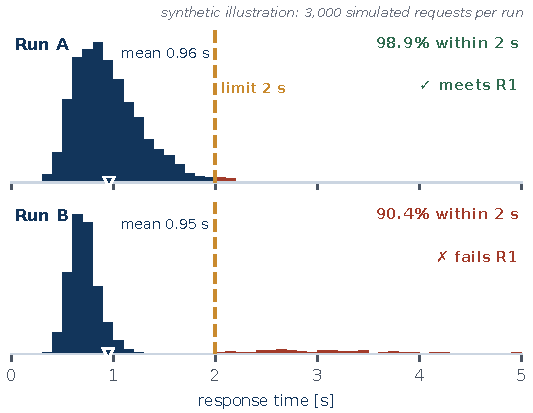
\includegraphics[height=5.3cm,keepaspectratio]{images/class22_latency_runs.pdf}
\column{0.45\textwidth}
\begin{tikzpicture}
\badge{0.05}{-0.4}{courseblue}{calculator}
\node[anchor=west, text width=5.3cm, align=left, font=\footnotesize] at (0.55,-0.4) {Both runs average about \textbf{one second}.};
\badge{0.05}{-1.35}{coursegold}{stopwatch}
\node[anchor=west, text width=5.3cm, align=left, font=\footnotesize] at (0.55,-1.35) {R1 asks for 95\% within 2 s: run~A \textbf{passes}, run~B \textbf{fails} because of its tail.};
\badge{0.05}{-2.4}{coursegreen}{pencil-alt}
\node[anchor=west, text width=5.3cm, align=left, font=\footnotesize] at (0.55,-2.4) {Name the statistic in the requirement: a share or a percentile, not an average.};
\node[tileblue, anchor=north west, minimum width=6.2cm, text width=5.8cm, align=left, font=\scriptsize] at (0,-3.2) {\textbf{\color{courseblue}Percentile.} The 95th percentile (p95) is the value below which 95\% of requests fall. ``p95 $\le$ 2 s'' and ``95\% within 2 s'' say the same thing.};
\end{tikzpicture}
\end{columns}
\coursefooter
\end{cframe}

\begin{cframe}{A user story needs acceptance criteria}{\cterm{User story}{one sentence stating a need as role, goal, and benefit.}\cterm{Given--When--Then}{acceptance criteria as starting state, action, expected result.}\cterm{Boundary case}{an input at the edge of what is allowed.}}
\centering
\begin{tikzpicture}
\node[tileblue, anchor=north west, minimum width=8.3cm, minimum height=1.35cm, text width=7.9cm, align=left, font=\footnotesize] at (0,0) {{\bfseries\scriptsize\goldink USER STORY}\\As a \textbf{\color{courseblue}support operator}, I want to \textbf{\color{coursegold!65!black}correct a suggested category} so that \textbf{\color{coursegreen}the ticket reaches the right team}.};
\node[font=\tiny\bfseries, text=coursegray, anchor=west] at (0,-1.6) {ACCEPTANCE CRITERION (GIVEN, WHEN, THEN)};
\foreach \y/\col/\lab/\txt in {-1.9/courseblue/GIVEN/a ticket with a suggested category, -2.75/coursegold/WHEN/the operator selects another approved category and confirms, -3.6/coursegreen/THEN/the system saves the selected category and records that an override occurred} {
  \node[rounded corners=3pt, fill=\col, text=white, anchor=north west, minimum width=1.4cm, minimum height=0.75cm, font=\scriptsize\bfseries] at (0,\y) {\lab};
  \node[tile, anchor=north west, minimum width=6.8cm, minimum height=0.75cm, text width=6.5cm, align=left, font=\scriptsize] at (1.5,\y) {\txt};
}
\ticketmock{8.9}{0}{1}
\node[note, anchor=north] at (11.3,-4.18) {Mock-up: the operator overrides the suggestion.};
\node[tilegold, anchor=north west, minimum width=13.4cm, minimum height=0.7cm, text width=12.6cm, align=left, font=\scriptsize] at (0,-4.65) {{\bfseries\goldink\faIcon{lightbulb}\ Key idea.}\ A story gives the why; the criteria give the proof. Cover failure and boundary cases, and describe the result without prescribing the implementation.};
\end{tikzpicture}
\coursefooter
\end{cframe}

\begin{cframe}{ML quality needs an evaluation contract}{\cterm{Macro-F1}{F1 computed for each category, then averaged with equal weight.}\cterm{Data leakage}{information from the test data reaching training, which inflates the score.}}
\centering
\begin{tikzpicture}
\node[tilegreen, anchor=north west, minimum width=13.4cm, minimum height=1.25cm, text width=12.6cm, align=left, font=\footnotesize] at (0,0) {{\bfseries\color{coursegreen}R2} \itshape Before release, macro-F1 shall be at least 0.80 on a held-out set of 1,000 manually labeled tickets sampled from the previous month, with no tickets from the same conversation in training.};
\node[anchor=north west, font=\tiny\bfseries, text=coursegray] at (0,-1.55) {AN EVALUATION CONTRACT NAMES FIVE THINGS};
\foreach \x/\ico/\name/\txt in {0/tags/Labels/{manually labeled tickets}, 2.7/inbox/Population/{1,000 tickets from the previous month}, 5.4/chart-bar/Metric/{macro-F1}, 8.1/flag/Threshold/{at least 0.80}, 10.8/filter/Procedure/{held out; conversations kept apart}} {
  \node[tileblue, anchor=north west, minimum width=2.6cm, minimum height=1.75cm] at (\x,-1.95) {};
  \node[circle, fill=courseblue, text=white, minimum size=0.55cm, inner sep=0, font=\footnotesize] at (\x+0.42,-2.28) {\faIcon{\ico}};
  \node[anchor=west, font=\scriptsize\bfseries, text=courseblue] at (\x+0.8,-2.28) {\name};
  \node[anchor=north west, text width=2.3cm, align=left, font=\scriptsize] at (\x+0.15,-2.6) {\txt};
}
\node[tile, anchor=north west, minimum width=4.3cm, minimum height=1.6cm, text width=3.95cm, align=left, font=\scriptsize] at (0,-3.85) {\textbf{\color{courseblue}Macro-F1.} Per-category F1 (a balance of precision and recall), averaged with equal weight: rare categories count as much as common ones.};
\node[tilered, anchor=north west, minimum width=4.3cm, minimum height=1.6cm, text width=3.95cm, align=left, font=\scriptsize] at (4.55,-3.85) {\textbf{\color{coursered}Leakage.} Tickets from one conversation are near-duplicates. Split across training and test, they inflate the score.};
\node[tilegold, anchor=north west, minimum width=4.3cm, minimum height=1.6cm, text width=3.95cm, align=left, font=\scriptsize] at (9.1,-3.85) {\textbf{\goldink Offline is not online.} A pass on last month's tickets does not guarantee future performance: the data may drift.};
\end{tikzpicture}
\coursefooter
\end{cframe}

\begin{cframe}{Specify uncertainty and failure behavior}{\cterm{ML model}{the trained classifier that maps a ticket to a category.}\cterm{Fallback}{behavior when the preferred path is unavailable.}\cterm{Abstention}{declining to answer when unsure.}}
\centering
\begin{tikzpicture}
\ticketmock{0}{0}{2}
\node[note, anchor=north] at (2.4,-4.15) {Mock-up: the scoring service is down.};
\node[tileblue, anchor=north west, minimum width=4.8cm, text width=4.4cm, align=left, font=\scriptsize] at (0,-4.65) {{\bfseries\color{courseblue}\faIcon{robot}\ ML model.} The trained classifier that suggests a category for a ticket. The \textbf{scoring service} is the program that runs it.};
\node[tileblue, anchor=north west, minimum width=8.3cm, minimum height=2.2cm, text width=7.9cm, align=left, font=\footnotesize] at (5.3,0) {{\bfseries\color{courseblue}Three questions to answer in the requirements}\\[2pt]\faIcon{exclamation-circle}\ What happens when the input is missing or too long?\\\faIcon{plug}\ What happens when the ML model is unavailable?\\\faIcon{hand-paper}\ When the model is unsure, can the system defer to a human instead of guessing a category?};
\node[tilegreen, anchor=north west, minimum width=8.3cm, minimum height=1.25cm, text width=7.9cm, align=left, font=\footnotesize] at (5.3,-2.4) {{\bfseries\color{coursegreen}R3 fallback.} \itshape If the scoring service is unavailable, the interface shall display ``Suggestion unavailable'' and allow the operator to route the ticket manually.};
\node[tilegold, anchor=north west, minimum width=8.3cm, minimum height=0.85cm, text width=7.9cm, align=left, font=\footnotesize] at (5.3,-3.85) {\faIcon{flask}\ {\bfseries\goldink Acceptance check.} Simulate a scoring-service outage and verify that manual routing still works.};
\node[tilegold, fill=white, anchor=north west, minimum width=8.3cm, minimum height=0.95cm, text width=7.9cm, align=left, font=\scriptsize] at (5.3,-5.0) {{\bfseries\goldink\faIcon{lightbulb}\ Key idea.} A wrong ML answer looks like a right one: say what happens when the model is absent, unsure, or wrong.};
\end{tikzpicture}
\coursefooter
\end{cframe}

% ================================================================== PART 3
\sectiondivider{3}{Validate and manage requirements}{balance-scale}{a requirement states a condition, an outcome, a threshold, and the evidence.}{$\bullet$\ Discover missing requirements before implementation\\[3pt]$\bullet$\ Make conflicts and priorities explicit\\[3pt]$\bullet$\ An example requirement form (IEEE style), and what changes\\[3pt]$\bullet$\ Review requirements with five questions}

\begin{cframe}{Discover missing requirements before implementation}{\cterm{Tacit knowledge}{what experts know and do but cannot easily put into words.}\cterm{Prototype}{a rough, quick version used to get feedback early.}\cterm{Ambiguous category}{a ticket that could belong to more than one category.}}
\renewcommand{\discchipw}{4.0}
\centering
\begin{tikzpicture}
\fill[coursegold!12] (9.65,-4.1) rectangle (13.7,0.55);
\node[anchor=west, font=\scriptsize\bfseries, text=coursegray] at (0,0.25) {TECHNIQUE};
\node[anchor=west, font=\scriptsize\bfseries, text=coursegray] at (4.2,0.25) {WHAT WE DO OR ASK};
\node[anchor=west, font=\scriptsize\bfseries, text=coursegold!65!black] at (9.75,0.25) {WHAT IT EXPOSES};
\discrow{-0.4}{comments}{Interview and observe}{Interview operators and watch how tickets are routed today.}{The real practice, and its workarounds}
\discrow{-1.2}{exclamation-triangle}{Cost of errors}{Ask which routing errors are most costly and which categories are ambiguous.}{Priorities and hard cases}
\discrow{-2.0}{tags}{Label ownership}{Check who defines the labels and resolves disagreements.}{Who owns the ground truth}
\discrow{-2.8}{lock}{Data and privacy}{Ask which ticket data may be displayed, stored, and accessed.}{Privacy and access rules}
\discrow{-3.6}{pencil-ruler}{Prototype walk-through}{Walk through a simple prototype with operators.}{Hidden assumptions}
\keyidea{-4.3}{Use several techniques: stakeholders cannot always say what they know (tacit knowledge), so observation and prototypes reveal what interviews miss.}
\end{tikzpicture}
\coursefooter
\end{cframe}

\begin{cframe}{Make conflicts and priorities explicit}{\cterm{Stakeholder conflict}{two needs or goals that cannot both be fully satisfied.}\cterm{Decision record}{a short note of what was decided, by whom, and why.}\cterm{Priority}{the order in which requirements matter when time is short.}}
\centering
\begin{tikzpicture}
\node[tilered, anchor=north west, minimum width=13.4cm, minimum height=0.8cm, text width=12.6cm, align=left, font=\footnotesize] at (0,0) {{\bfseries\color{coursered}\faIcon{balance-scale}\ Example conflict.} Automatically routing more tickets may reduce manual work while increasing incorrect routing.};
\node[anchor=north west, inner sep=0] at (0,-1.0) {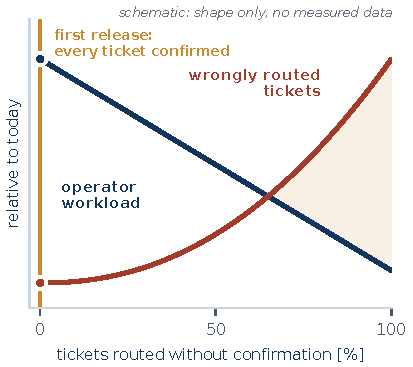
\includegraphics[height=4.0cm]{images/class22_automation_tradeoff.pdf}};
\node[tileblue, anchor=north west, minimum width=8.3cm, minimum height=3.95cm] at (5.1,-1.0) {};
\foreach \y/\n/\lab/\txt in {-1.2/1/AGREE/{which errors matter most, and who accepts the trade-off.}, -1.95/2/DECIDE/{for example, keep operator confirmation for every ticket in the first release.}, -2.7/3/RECORD/{the decision, its owner, and the evidence needed to revisit it.}} {
  \node[circle, fill=coursegold, text=white, font=\tiny\bfseries, minimum size=0.42cm, inner sep=0] at (5.4,\y-0.25) {\n};
  \node[anchor=north west, text width=7.3cm, align=left, font=\scriptsize] at (5.7,\y) {{\bfseries\color{courseblue}\lab:} \txt};
}
\node[anchor=north west, font=\tiny\bfseries, text=coursegray] at (5.3,-3.55) {PRIORITIZE};
\node[tilegreen, anchor=north west, minimum width=3.7cm, minimum height=0.85cm, text width=3.4cm, align=left, font=\scriptsize] (essential) at (5.3,-3.9) {{\bfseries\color{coursegreen}Essential:} manual fallback};
\node[tile, anchor=north west, minimum width=3.7cm, minimum height=0.85cm, text width=3.4cm, align=left, font=\scriptsize] (optional) at (9.55,-3.9) {{\bfseries\color{courseblue}Optional:} convenience features};
\draw[arrowgold] (essential.east) -- (optional.west);
\end{tikzpicture}
\coursefooter
\end{cframe}

\begin{cframe}{Example: a requirement form in the IEEE style}{\cterm{SRS}{Software Requirements Specification, the document that lists a system's requirements.}\cterm{Verification method}{how a requirement is checked: test, demonstration, inspection, or analysis.}\cterm{Traceability}{links from a need to a requirement to its check.}}
\centering
\begin{tikzpicture}
\filldraw[fill=white, draw=courseblue!55, thick, rounded corners=4pt] (0,0) rectangle (8.6,-4.4);
\fill[courseblue, rounded corners=4pt] (0,0) rectangle (8.6,-0.55);
\fill[courseblue] (0,-0.3) rectangle (8.6,-0.55);
\node[anchor=west, text=white, font=\small\bfseries] at (0.2,-0.275) {\faIcon{file-signature}\ Requirement record};
\node[tag, anchor=east] at (8.4,-0.275) {EXAMPLE: HYPOTHETICAL VALUES};
\formrow{-0.55}{0.45}{ID AND TITLE}{\textbf{R1} \ Suggestion latency \ {\color{coursegray}(non-functional)}}
\formrow{-1.0}{1.05}{STATEMENT}{With 20 concurrent users and ticket bodies up to 5,000 characters, at least 95\% of suggestion requests \textbf{shall} complete within 2 seconds.}
\formrow{-2.05}{0.7}{RATIONALE}{Operators route tickets while customers wait; slow suggestions would be ignored.}
\formrow{-2.75}{0.45}{SOURCE}{Support operators (interviews)}
\formrow{-3.2}{0.45}{PRIORITY}{High, to be negotiated \quad|\quad Status: proposed}
\formrow{-3.65}{0.75}{VERIFICATION}{\textbf{Test:} a 30-minute load test; passes if at least 95\% of requests finish within 2 s.}
\node[tileblue, anchor=north west, minimum width=4.85cm, text width=4.5cm, align=left, font=\scriptsize] at (8.8,0) {{\bfseries\color{courseblue}\faIcon{landmark}\ Where it comes from}\\[2pt]ISO/IEC/IEEE 29148 (2018) replaced IEEE 830-1998. Its SRS template groups requirements by kind and ends with verification.};
\node[tilegold, anchor=north west, minimum width=4.85cm, text width=4.5cm, align=left, font=\scriptsize] at (8.8,-2.2) {{\bfseries\goldink\faIcon{vial}\ Four verification methods}\\[2pt]\textbf{Test:} run it and measure (R1).\\\textbf{Demonstration:} operate, observe.\\\textbf{Inspection:} examine an artifact.\\\textbf{Analysis:} calculate or reason.};
\keyidea{-4.7}{A form makes every requirement carry its rationale, source, priority, and verification method: the data needed for traceability, negotiation, and change control.}
\end{tikzpicture}
\coursefooter
\end{cframe}

\begin{cframe}{When something changes: use the traces to find the impact}{\cterm{Impact analysis}{finding everything a proposed change touches before approving it.}\cterm{Volatile requirement}{one likely to change, such as a category list.}}
\centering
\begin{tikzpicture}
\node[tilegold, minimum width=3.0cm, minimum height=1.7cm, text width=2.7cm, font=\small] (change) at (1.5,-2.15) {{\Large\goldink\faIcon{tags}}\\[2pt]\textbf{The category taxonomy changes}};
\foreach \i/\y/\ico/\name/\txt in {1/0/tags/Labels/{Do existing labels still fit the new list?}, 2/-1.1/database/Evaluation data/{Does the held-out set still cover every category?}, 3/-2.2/desktop/Interface choices/{Do menus and fallbacks show the new list?}, 4/-3.3/clipboard-check/Acceptance tests/{Do the load, evaluation, and outage tests apply?}} {
  \node[tileblue, anchor=north west, minimum width=6.6cm, minimum height=0.95cm] (imp\i) at (4.0,\y) {};
  \node[circle, fill=courseblue, text=white, minimum size=0.6cm, inner sep=0, font=\footnotesize] at (4.4,\y-0.48) {\faIcon{\ico}};
  \node[anchor=west, text width=5.7cm, align=left, font=\scriptsize] at (4.85,\y-0.48) {{\bfseries\color{courseblue}\name.} \txt};
}
\node[tilegreen, minimum width=2.6cm, minimum height=1.7cm, text width=2.3cm, font=\small] (approve) at (12.3,-2.15) {{\Large\color{coursegreen}\faIcon{check-circle}}\\[2pt]\textbf{Approve the new version}};
\foreach \i in {1,2,3,4} {
  \draw[arrowgold] (change.east) to[out=0, in=180] (imp\i.west);
  \draw[arrowgreen] (imp\i.east) to[out=0, in=180] (approve.west);
}
\node[font=\tiny\bfseries, text=coursegray] at (7.3,0.3) {REVIEW BEFORE APPROVING};
\keyidea{-4.55}{Impact analysis is only possible if the links exist: each requirement connects to a need, to the data it depends on, and to a check.}
\end{tikzpicture}
\coursefooter
\end{cframe}

\begin{cframe}{Review requirements with five questions}{\cterm{Feasible}{achievable with the available data, time, and resources.}\cterm{Verification}{checking that the system meets its requirements.}}
\centering
\begin{tikzpicture}
\foreach \y/\ico/\name/\q in {-0.45/user-check/Necessary/{Whose need does this support?}, -1.3/search/Unambiguous/{Could two readers interpret it differently?}, -2.15/flask/Testable/{What evidence would establish that it passes?}, -3.0/tools/Feasible/{Do the data, time, and resources support it?}, -3.85/link/Traceable/{Can we connect it to a need, a test, and future changes?}} {
  \node[chip, anchor=west, minimum width=3.7cm, minimum height=0.72cm, font=\small\bfseries] at (0,\y) {\faIcon{\ico}\ \name};
  \node[anchor=west, font=\normalsize, text width=9.6cm, align=left] at (4.0,\y) {\q};
  \draw[courseice!70!courseblue, line width=0.5pt] (0,\y-0.47) -- (13.7,\y-0.47);
}
\node[tile, anchor=north west, minimum width=13.4cm, minimum height=0.95cm, text width=12.8cm, align=left, font=\footnotesize] at (0,-4.5) {\textbf{\color{courseblue}Validation} of requirements asks: are these the right requirements? \textbf{\color{courseblue}Verification} asks: does the built system meet them? This review is validation; the acceptance checks are verification.};
\end{tikzpicture}
\coursefooter
\end{cframe}

\begin{frame}{Three ideas to keep}
\centering
\begin{tikzpicture}
\foreach \x/\ico/\title/\txt in {0/link/Need to check/A requirement connects a stakeholder need to a result that can be checked., 4.55/flask/More than a model score/ML requirements cover evaluation conditions and human fallback as well as model scores., 9.1/file-signature/Write it down/{Write down priorities, acceptance evidence, and the impact of changes.}} {
  \node[tileblue, anchor=north west, minimum width=4.3cm, minimum height=4.1cm] at (\x,0) {};
  \node[circle, fill=courseblue, text=white, minimum size=1.2cm, inner sep=0, font=\Large] at (\x+2.15,-0.85) {\faIcon{\ico}};
  \node[font=\small\bfseries, text=courseblue, text width=3.9cm, align=center] at (\x+2.15,-1.85) {\title};
  \node[anchor=north west, text width=3.9cm, align=left, font=\footnotesize] at (\x+0.2,-2.3) {\txt};
}
\node[tilegold, anchor=north west, minimum width=13.4cm, minimum height=1.35cm, text width=12.4cm, align=left, font=\footnotesize] at (0,-4.4) {{\bfseries\goldink\faIcon{book-open}\ Further reading.} Sommerville, \textit{Software Engineering}: requirements engineering. User stories and acceptance criteria in the \href{https://www.atlassian.com/agile/project-management/user-stories}{Atlassian guide}.};
\end{tikzpicture}
\coursefooter
\end{frame}

% ------------------------------------------------------------------ application: requirements as prompts
\section{Application}\gdef\currentsectionname{Application}
\begin{cframe}{AI-assisted programming: a good prompt is a good requirement}{\cterm{AI-assisted programming}{coding with an assistant that generates code.}\cterm{Hidden assumption}{a gap the model fills with a guess.}}
\centering
\begin{tikzpicture}
\fill[coursegold!12] (9.65,-4.15) rectangle (13.7,0.55);
\node[anchor=west, font=\scriptsize\bfseries, text=coursegray] at (0,0.3) {GOOD REQUIREMENT};
\node[anchor=west, font=\scriptsize\bfseries, text=coursegray] at (3.5,0.3) {BECOMES, IN THE PROMPT};
\node[anchor=west, font=\scriptsize\bfseries, text=coursegold!65!black] at (9.75,0.3) {WHY IT HELPS};
\discrow{-0.45}{user-check}{Necessary}{Need and scope: who uses it, what it must do, and what not to build or change.}{Stops over-building and unwanted edits.}
\discrow{-1.25}{search}{Unambiguous}{One \texttt{shall} statement per line, with an ID, a threshold, and the behavior on failure.}{Checkable lines and fewer hidden guesses.}
\discrow{-2.05}{flask}{Testable}{``Write the tests first (Given--When--Then), run them, and report failures.''}{``Looks right'' becomes pass or fail.}
\discrow{-2.85}{tools}{Feasible}{Limits and resources: language, libraries, data, and performance targets.}{Fewer invented APIs and impossible targets.}
\discrow{-3.65}{link}{Traceable}{``Cite the requirement ID in each change; list any requirement not covered.''}{The diff can be reviewed against the spec.}
\keyidea{-4.45}{Review the prompt with the same five questions, and keep the spec in the repository. The assistant fills every gap with a guess; checking stays your job.}
\end{tikzpicture}
\coursefooter
\end{cframe}

% ------------------------------------------------------------------ closing
\section{Wrap-up}\gdef\currentsectionname{Wrap-up}
\begin{frame}{From this class to the next}
\centering
\begin{tikzpicture}
\foreach \i/\lab/\bg/\fg in {1/SE and ML/courseblue!22/courseblue, 2/Requirements/courseblue/white, 3/Process/coursegold/white, 4/Design/courseice/coursegray, 5/Quality/courseice/coursegray, 6/Evolution/courseice/coursegray} {
  \node[rounded corners=3pt, minimum width=2.18cm, minimum height=0.6cm, font=\scriptsize\bfseries, fill=\bg, text=\fg] at ({1.1+(\i-1)*2.28},0) {\i\ \lab};
}
\node[font=\tiny\bfseries, text=courseblue] at (3.38,-0.52) {THIS CLASS};
\node[font=\tiny\bfseries, text=coursegold!70!black] at (5.66,-0.52) {NEXT: CLASS 23};
\foreach \x/\sty/\ico/\ttl/\txt in {0/tileblue/lightbulb/What stays with us/{$\bullet$\ A requirement links a need to a result that can be checked.\\[3pt]$\bullet$\ ML adds evaluation conditions and a fallback.\\[3pt]$\bullet$\ A good prompt is a good requirement.}, 4.55/tileblue/project-diagram/Use it in your project/{$\bullet$\ Give each requirement an ID, a threshold, and a check.\\[3pt]$\bullet$\ Record rationale, source, and priority.\\[3pt]$\bullet$\ Say what happens when the model fails.}, 9.1/tilegold/arrow-right/Next: Class 23/{\textbf{Process Models and Agile Foundations.}\\[3pt]How teams organize work across exploration, validation, and release, especially when requirements may change.}} {
  \node[\sty, anchor=north west, minimum width=4.3cm, minimum height=4.1cm] at (\x,-0.95) {};
  \badge{\x+0.65}{-1.6}{courseblue}{\ico}
  \node[anchor=west, text width=3.0cm, align=left, font=\small\bfseries, text=courseblue] at (\x+1.2,-1.6) {\ttl};
  \node[anchor=north west, text width=3.9cm, align=left, font=\scriptsize] at (\x+0.2,-2.25) {\txt};
}
\node[tilegold, fill=white, anchor=north west, minimum width=13.4cm, minimum height=0.95cm, text width=12.6cm, align=left, font=\footnotesize] at (0,-5.25) {{\bfseries\goldink\faIcon{route}\ Course thread.} Knowing what ``good'' means before we build now leads to how we organize the work (Class 23) and, later, how we run it in production (MLOps).};
\end{tikzpicture}
\coursefooter
\end{frame}

% ------------------------------------------------------------------ references
\begin{frame}{References}
\centering
\begin{tikzpicture}
\refrow{0}{0.8}{book}{Textbook}{Sommerville, I. \href{https://www.pearson.com/en-us/subject-catalog/p/software-engineering/P200000003144/9780137035151}{\emph{Software Engineering}}, Pearson: the requirements engineering chapters.}
\refrow{-0.8}{1.25}{landmark}{Standards}{ISO/IEC/IEEE 29148:2018. \href{https://www.iso.org/standard/72089.html}{Systems and software engineering: Life cycle processes: Requirements engineering}.\\[3pt]It replaced \href{https://standards.ieee.org/standard/830-1998.html}{IEEE Std 830-1998}, the earlier SRS recommended practice.}
\refrow{-2.05}{1.55}{robot}{Requirements for ML}{Vogelsang, A. and Borg, M. (2019). \href{https://arxiv.org/abs/1908.04674}{Requirements Engineering for Machine Learning: Perspectives from Data Scientists}. IEEE RE Workshops.\\[3pt]Nahar, N. et al. \href{https://arxiv.org/abs/2110.10234}{Collaboration Challenges in Building ML-Enabled Systems} (arXiv:2110.10234).}
\refrow{-3.6}{1.25}{clipboard-check}{Stories and criteria}{Atlassian. \href{https://www.atlassian.com/agile/project-management/user-stories}{User stories: examples and a template}.\\[3pt]North, D. (2006). \href{https://dannorth.net/introducing-bdd/}{Introducing BDD}: behavior-driven development and the Given--When--Then format.}
\end{tikzpicture}
\coursefooter
\end{frame}

\end{document}
